\documentclass[a4paper,twoside]{article}
\usepackage[T1]{fontenc}
\usepackage[bahasa]{babel}
\usepackage{graphicx}
\usepackage{graphics}
\usepackage{float}
\usepackage[cm]{fullpage}
\pagestyle{myheadings}
\usepackage{etoolbox}
\usepackage{setspace} 
\usepackage{lipsum} 
\setlength{\headsep}{30pt}
\usepackage{caption}
\usepackage{hyperref}
\usepackage{multirow}
\usepackage{longtable}
\usepackage{array}
\usepackage{hyperref}
\usepackage[inner=2cm,outer=2.5cm,top=2.5cm,bottom=2cm]{geometry} %margin
% \pagestyle{empty}

\makeatletter
\renewcommand{\@maketitle} {\begin{center} {\LARGE \textbf{ \textsc{\@title}} \par} \bigskip {\large \textbf{\textsc{\@author}} }\end{center} }
\renewcommand{\thispagestyle}[1]{}
\markright{\textbf{\textsc{Laporan Perkembangan Pengerjaan Skripsi\textemdash Sem. Genap 2022/2023}}}

\onehalfspacing
 
\begin{document}

\title{\@judultopik}
\author{\nama \textendash \@npm} 

%ISILAH DATA BERIKUT INI:
\newcommand{\nama}{Bosnich Timothy Bonsaleng}
\newcommand{\@npm}{2017730086}
\newcommand{\tanggal}{22/12/2023} %Tanggal pembuatan dokumen
\newcommand{\@judultopik}{Pemvisualisasi Hasil Penelitian Area Hijau
	Kelurahan} % Judul/topik anda
\newcommand{\kodetopik}{PAN5491}
\newcommand{\jumpemb}{1} % Jumlah pembimbing, 1 atau 2
\newcommand{\pembA}{Pascal~Alfadian,~Nugroho,~M.Comp.}
\newcommand{\pembB}{-}
\newcommand{\semesterPertama}{54 - Genap 22/23} % semester pertama kali topik diambil, angka 1 dimulai dari sem Ganjil 96/97
\newcommand{\lamaSkripsi}{2} % Jumlah semester untuk mengerjakan skripsi s.d. dokumen ini dibuat
\newcommand{\kulPertama}{Skripsi 1} % Kuliah dimana topik ini diambil pertama kali
\newcommand{\tipePR}{C} % tipe progress report :
% A : dokumen pendukung untuk pengambilan ke-2 di Skripsi 1
% B : dokumen untuk reviewer pada presentasi dan review Skripsi 1
% C : dokumen pendukung untuk pengambilan ke-2 di Skripsi 2

% Dokumen hasil template ini harus dicetak bolak-balik !!!!

\maketitle

\pagenumbering{arabic}

\section{Data Skripsi} %TIDAK PERLU MENGUBAH BAGIAN INI !!!
Pembimbing utama/tunggal: {\bf \pembA}\\
Pembimbing pendamping: {\bf \pembB}\\
Kode Topik : {\bf \kodetopik}\\
Topik ini sudah dikerjakan selama : {\bf \lamaSkripsi} semester\\
Pengambilan pertama kali topik ini pada : Semester {\bf \semesterPertama} \\
Pengambilan pertama kali topik ini di kuliah : {\bf \kulPertama} \\
Tipe Laporan : {\bf \tipePR} -
\ifdefstring{\tipePR}{A}{
			Dokumen pendukung untuk {\BF pengambilan ke-2 di Skripsi 1} }
		{
		\ifdefstring{\tipePR}{B} {
				Dokumen untuk reviewer pada presentasi dan {\bf review Skripsi 1}}
			{	Dokumen pendukung untuk {\bf pengambilan ke-2 di Skripsi 2}}
		}
		
\section{Latar Belakang}
Ruang Terbuka Hijau merupakan suatu ruang terbuka di kawasan perkotaan yang didominasi tutupan lahannya oleh unsur hijau (vegetasi) serta memiliki fungsi antara lain sebagai area untuk rekreasi, sosial budaya, estetika, ekologis dan dapat memberikan nilai ekonomis bagi perkembangan suatu wilayah perkotaan (lihat Gambar \ref{fig:rth}). Definisi RTH sendiri dalam pasal 1 UU No.26/2007 tentang Penataan Ruang adalah area memanjang/jalur dan/atau mengelompok, yang penggunaannya lebih bersifat terbuka, tempat tumbuh tanaman, baik yang tumbuh secara alamiah maupun yang sengaja ditanam. Pada pasal 29 disebutkan bahwa ruang terbuka hijau terdiri dari ruang terbuka hijau publik dan ruang terbuka hijau privat, dimana proporsi ruang terbuka hijau kota paling sedikit 30\% dari luas wilayah kota, sedangkan proporsi ruang terbuka hijau publik paling sedikit 20\% dari luas wilayah kota. %jgn lupa referensi

\begin{figure}[h]
	\centering
	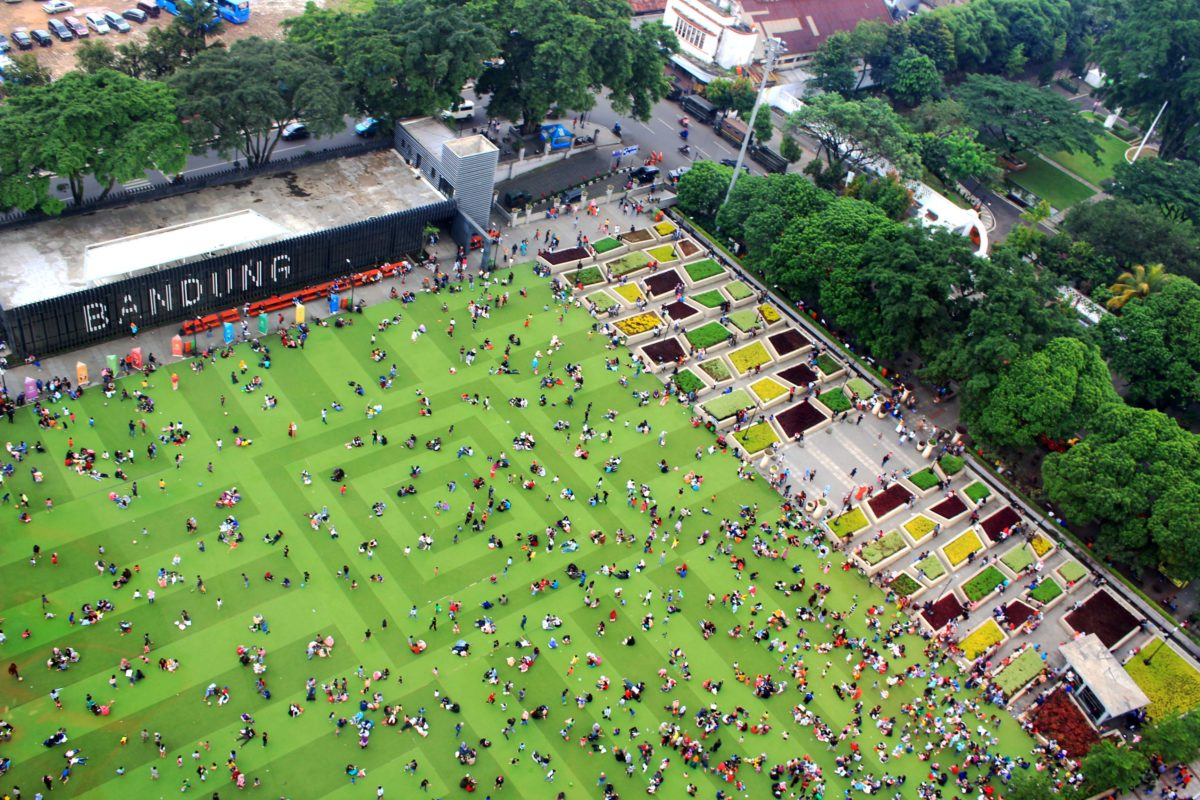
\includegraphics[width=0.7\textwidth]{ruang terbuka hijau.jpg}
	\caption[RTH]{Contoh Ruang Terbuka Hijau\protect\footnotemark}
	\label{fig:rth}
\end{figure}

\footnotetext{Ilustrasi ruang terbuka hijau: \url{https://www.rth.bandung.go.id/}}



Pemanfaatan citra satelit merupakan sebuah cara agar dapat mengetahui luas RTH pada suatu kota. Citra Satelit adalah gambaran dari permukaan bumi yang didapatkan langsung dari satelit. Oleh karena itu, citra satelit dapat digunakan dalam mengidentifikasi RTH yang mana terdapatnya banyak pepohonan pada suatu wilayah. Perhitungan juga dapat dilakukan pada citra satelit ,dan hasil dari perhitungan luas RTH pada suatu wilayah diharapkan dapat memberikan dorongan untuk peningkatan dalam penghijauan agar dapat digunakan oleh pemerintah dalam merancang dan meningkatkan penghijauan di berbagai wilayah di Indonesia.

Penelitian yang dilakukan oleh Juan A. Kusjadi yaitu mengimplementasikan program untuk mengumpulkan, menyiapkan, dan menganalisis data
citra satelit kelurahan dari beberapa kota/kabupaten di Indonesia menggunakan Hadoop MapReduce. Data kemudian disimpan pada sistem data lake yang telah dibuat pada Hadoop HDFS. Data hasil analisis dan perhitungan luas RTH juga sudah dilakukan evaluasi dengan nilai sesungguhnya. Data hasil penelitian akan digunakan sebagai penunjang dalam pembuatan halaman web. 

Pada Skripsi ini, akan dibangun sebuah halaman web yang interaktif yaitu pemvisualisasian dari hasil penelitian area hijau Kota Bandung. Visualisasi adalah rekayasa dalam pembuatan gambar, diagram atau animasi untuk penampilan suatu informasi dalam penjelasan lain visualisasi adalah konversi data ke dalam format visual atau tabel sehingga karakteristik dari data dan relasi diantara item data atau atribut dapat di analisis atau dilaporkan, dan visualisasi data adalah satu dari yang teknik paling baik dan menarik untuk eksplorasi data. Manusia memiliki kemampuan membangun yang baik untuk menganalisis sejumlah besar informasi yang dipresentasi secara visual. Ia dapat mendeteksi pola umum dan trend, pencilan dan pola yang tidak umum. Oleh karena itu, dengan dikembangkannya halaman web ini memiliki tujuan agar para pengguna dapat mengetahui informasi yang terdapat pada kelurahan. Informasi yang terdapat pada halaman website berupa nama kelurahan, luas wilayah kelurahan, gambar dari keluruhan/kecamatan, dll. Informasi yang terkumpul akan digunakan untuk mengembangkan halaman web.
%Pressman, Roger S. 2002.”Rekayasa Perangkat Lunak (Pendekatan Praktis).” Yogyakarta : Andi


Halaman web yang akan dikembangkan harusnya dapat diakses melalui komputer atau laptop. Dalam pengembangan halaman web pemvisualisasi area hijau kota Bandung akan dibantu pembuatannya dengan menggunakan \emph{Framework} Laravel. Penggunaan \textit{Framework} Laravel untuk memudahkan pengembang untuk membangun halaman web, sehingga pengguna yang akan mengakses halaman web akan dimudahkan dalam melihat informasi kelurahan dengan cepat. 

Laravel merupakan \textit{framework} PHP yang menekankan pada kesederhanaan dan flesksibelitas pada desainnya. Keunggulan ini didapatkan karena Laravel menggunakan konsep MVC (Model View Controller). Model pada Laravel berguna untuk membantu pengembang berinteraksi dengan database mengunakan \textit{syntax migration} yang merupakan bawaan dari Laravel. Dengan \textit{migration}, pengembangan dapat dengan mudah untuk melakukan modifikasi sebuah database pada sebuah platform secara independen karena implementasi skemas \textit{database} yang direpresentasikan dalam sebuah class. View pada Laravel akan menjadi wadah tampilan website (\textit{frond-end}). Dan Controller yang berfungsi untuk merespon setiap request yang ada pada website sehingga setiap fungsi yang ada akan berfungsi sebagaimana mestinya. Dengan berbagai kemudahan dan fitur yang ada pada Laravel inilah yang membuat pemngembang ingin menggunakannya dalam membangun halaman web pemvisualisasian area hijau kelurahan kota Bandung.


Dalam proses pengembangan halaman web tentu saja dibutuhkan sebuah data. Data yang akan digunakan dalam pembentukan halaman web berupa gambar dari kelurahan di Kota Bandung. Tidak hanya berupa gambar dari kelurahan tetapi juga berupa luas area wilayah untuk mengetahui besar wilayah kelurahan, mengetahui luas wilayah hijau kelurahan, dan melihat kebutuhan area hijau terhadap kelurahan di Kota Bandung. Perhitungan luas wilayah, luas wilayah hijau, dan kebutuhan area hijau telah dilakukan perhitungan untuk setiap kelurahan yang ada. 

\begin{figure}[H]
	\centering
	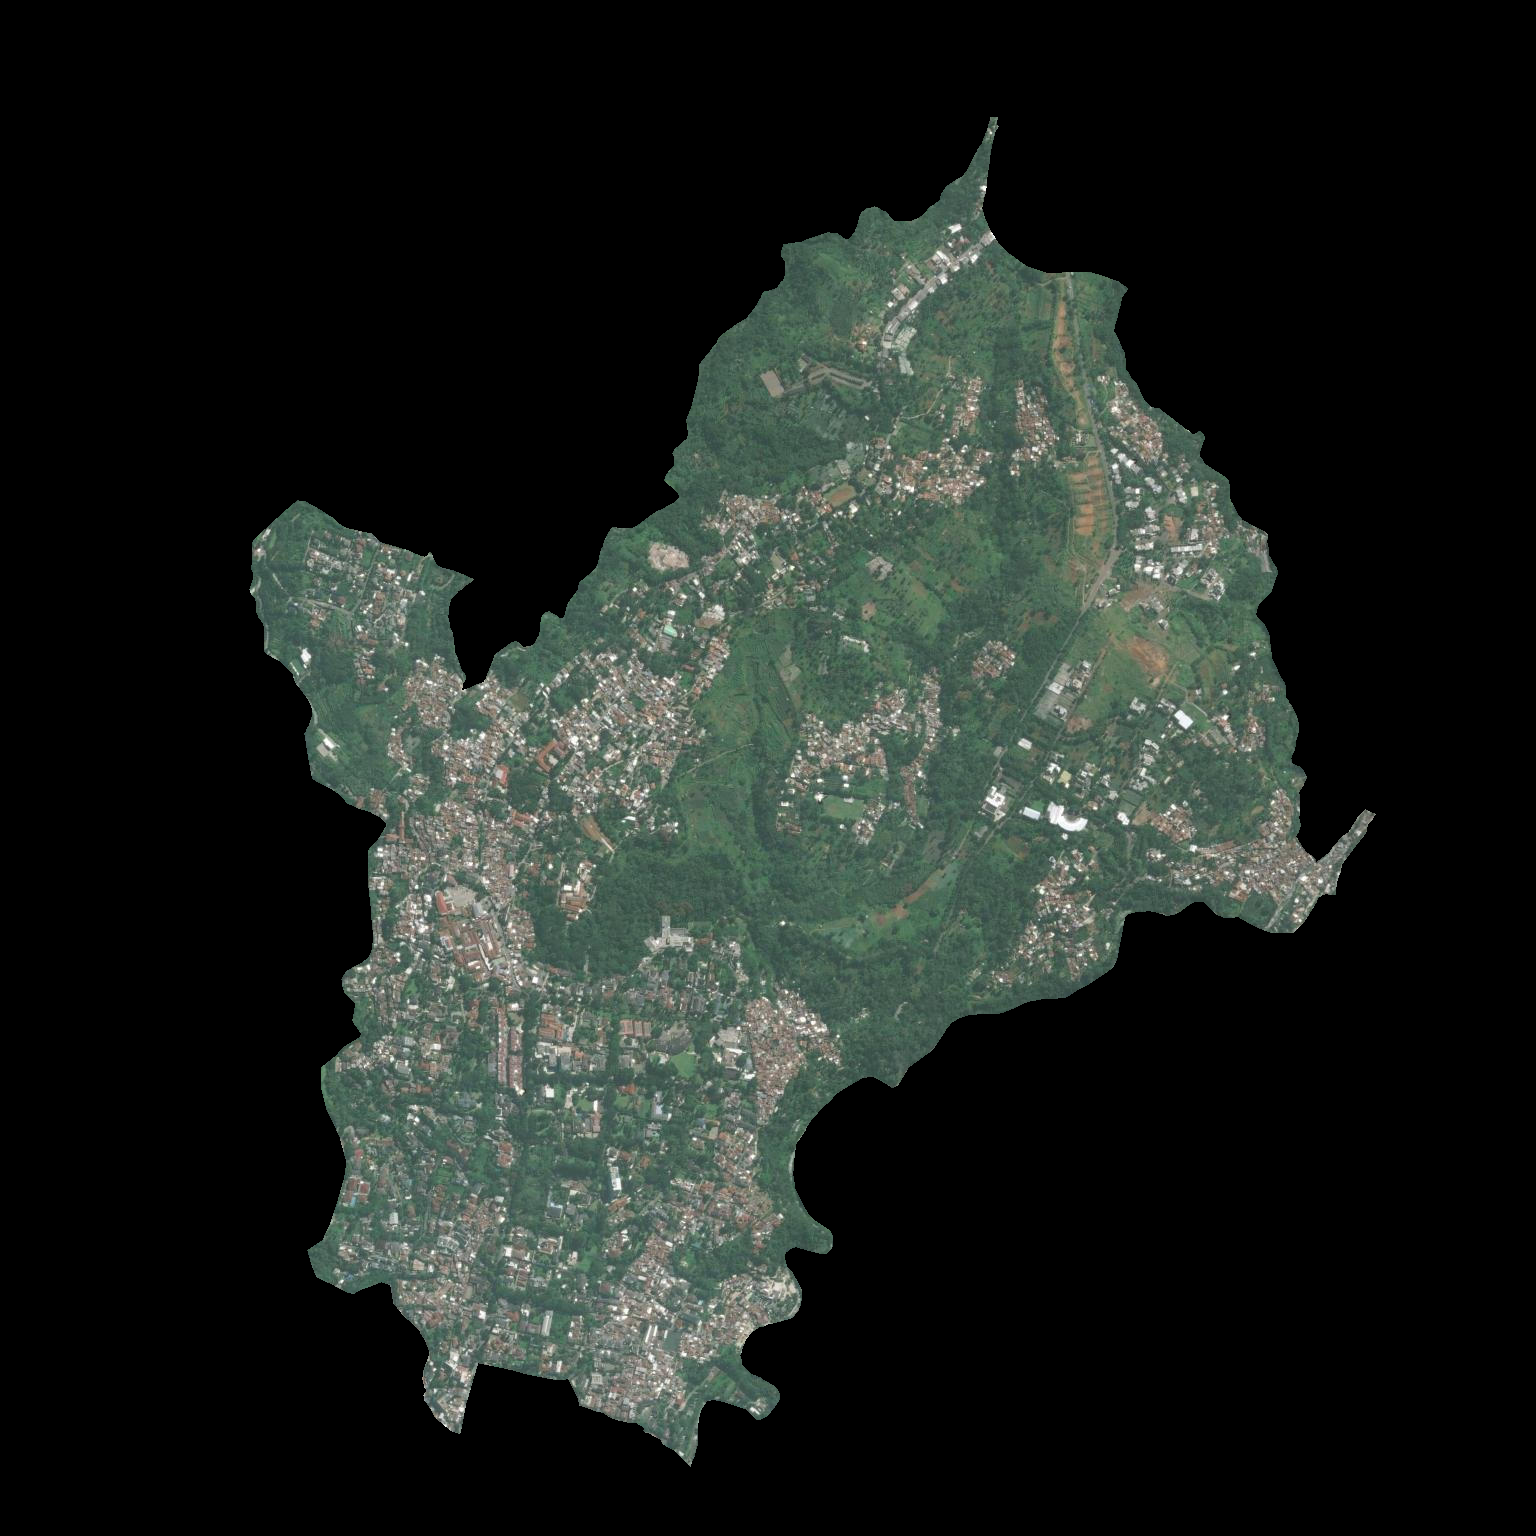
\includegraphics[width=0.6\textwidth]{Ciumbuleuit.png}
	\caption{Kelurahan Ciumbuleuit}
	\label{fig:ciumbuleuit}
\end{figure}



Contoh gambar dari hasil penelitian Juan A. Kusjadi dapat dilihat pada gambar \ref{fig:ciumbuleuit} yang mana merupakan hasil proses pengambilan gambar sebuah kelurahan Ciumbuleuit yang telah disimpan pada Hadoop HDFS. Proses pengambilan gambar dilakukan dengan menggunakan bahasa pemrograman Python\footnote{Python adalah bahasa pemrograman yang banyak digunakan dalam aplikasi web, pengembangan perangkat lunak, ilmu data, dan \textit{machine learning} (ML). Developer menggunakan Python karena efisien dan mudah dipelajari serta dapat dijalankan di berbagai platform.}. Berbagai macam \textit{library} yang dapat digunakan pada bahasa pemrograman Python dalam membantu pengembangan laman web, diantaranya menggunakan \textit{Python PIL(Pillow)} yang berguna untuk menggabungkan gambar, dan \textit{library} base 64 yang digunakan dalam melakukan peng-\textit{decode}-an teks yang merupakan sebuah \textit{tile} gambar kelurahan.

Hasil dari pemvisualisasi ruang terbuka hijau kelurahan pada kota Bandung akan menjadi sebuah halaman website yang interaktif yang dapat membandingkan kelurahan sesuai dengan masukan oleh pengguna. Dengan dikembangkan halaman website ini maka pengguna dapat memenuhi kebutuhan tempat tinggal bagi masyarakat agar dapat beraktivitas dengan normal dan mendapatkan kadar oksigen yang merata. 


\section{Rumusan Masalah}
Berdasarkan deskripsi dan latar belakang yang sudah dibahas bahwa rumusan masalah yang muncul adalah sebagai berikut:

\begin{enumerate}
	\item Bagaimana membuat sebuah halaman website interaktif yang dapat membandingkan data dua buah kelurahan Kota Bandung?
	\item Bagaimana cara pengguna untuk membandingkan atribut-atribut Citra Satelit dari kelurahan Kota Bandung?
	\item Bagaimana cara mengekstraksi data citra satelit pada HDFS ke \textit{local directory}?	
\end{enumerate}

\section{Tujuan}
Tujuan dari skripsi ini adalah:
\begin{enumerate}
	\item Membuat sebuah halaman website interaktif yang dapat membandingkan dua lokasi kelurahan.
	\item Pengguna dapat memilih kelurahan untuk sisi kiri dan kanan, untuk membandingkan atributnya.
	\item Data citra satelit yang didapatkan akan digunakan untuk memenuhi kebutuhan pada laman web yang akan dibangun.
\end{enumerate}

\section{Detail Perkembangan Pengerjaan Skripsi}
Detail bagian pekerjaan skripsi sesuai dengan rencana kerja/laporan perkembangan terkahir :
	\begin{enumerate}
		\item \textbf {Melakukan survei kepada Fritz H. Hutapea SKom dan Juan A. Kusjadi terkait penenilitiannya}\\
		{\bf Status :} Ada sejak rencana kerja skripsi.\\
		{\bf Hasil :} Survei sudah dilakukan sekali dengan Fritz~H.~Hutapea~Skom pada tanggal 12 Desember 2022. Melakukan wawancara melalui sosial media \textit{Instagram}, Hasil wawancara mengenai file peta kelurahan bandung geoJSON. Survei kedua dilakukan sekali dengan Juan~A.~Kusjadi pada tanggal 30 Januari 2023. Wawancara yang dilakukan melalui \textit{Google Meet}, Hasil wawancara yang dilakukan berbincang mengenai data citra satelit. Data citra satelit yang didapatkan dari penyimpanan hadoop pada lab UNPAR(Universitas Katholik Parahyangan) dan mendaptkan dokumentasi skripsi Juan~A.~Kusjadi yang digunakan sebagai referensi utama dalam pengembangan laman web.
		
		\item \textbf{ Melakukan pengumpulan data hasil penelitian}\\
		{\bf Status :} Ada sejak rencana kerja skripsi.\\
		{\bf Hasil :} Pengumpulan data yang dilakukan dengan cara mendaftarkan diri untuk mendapatkan akun untuk dapat mengakses penyimpanan \textit{hadoop} laboratorium FTIS UNPAR. Data hasil penelitian masih berupa format file ".txt" dan ".csv". Dari data hasil penilitian tersebut diunduh ke laptop pribadi melalui jaringan FTIS UNPAR. Data yang berupa format file ".txt" dapat diekstraksi menjadi sebuah gambar dari kelurahan atau kecamata Kota Bandung. Pengekstraksian data gambar dilakukan dengan menggunakan \textit{script python}. Dalam penggunaan \textit{script} terdapat beberapa \textit{library} dari bahasa pemrograman \textit{python} yaitu base64 digunakan untuk men-\textit{decode} data file menjadi format ".png" yang menghasilkan gambar berupa kumpulan \textit{tile} pembentuk gambar utuh dari kelurahan atau kecamatan dan \textit{Python PIL(Pillow)} sebagai penggabungan gambar dari kumpulan \textit{tile} menjadi sebuah gambar utuh dari kelurahan atau kecamatan. Proses pengumpulan data telah dilakukan pada bab 3, data kelurahan yang didapatkan dari hasil penelitian yang telah dilakukan oleh Juan A. Kusjadi. Data yang ditemukan merupakan hasil perhitungan luas wilayah kelurahan dan wilayah RTH kelurahan di Kota Bandung dengan menggunakan algoritma KMeans dengan k=5 dalam pendekatan \textit{pixel based}. Hasil dari penelitian tersebut didapat dari lampiran hasil eksperimen yang berisikan nama kelurahan, luas kelurahan sesungguhnya dalam satuan km2, luas kelurahan preidiksi dalam satuan km2, luas RTH kelurahan prediksi dalam satuan km2, dan persentase RTH kelurahan.
		
		
		\item \textbf{Melakukan studi literatur dan studi eksplorasi mengenai Apache Hadoop}\\
		{\bf Status :} Ada sejak rencana kerja skripsi.\\
		{\bf Hasil :} Pembelajaran mengenai studi literatur dan studi eksplorasi menghasilkan mengetahui \textit{Hadoop command-line} yang digunakan dalam pengunduhan data dari laboratoium FTIS UNPAR. Perintah-perintah yang digunakan dalam HDFS seperti :
		\begin{itemize}
			\item Penggunaan perintah \textbf{dfs}\\
			Perintah \textbf{dfs} digunakan untuk menjalankan(\textit{run}) perintah \textit{filesystem} yang didukung oleh \textit{Hadoop}. \textit{\textbf{[COMMAND\_OPTIONS]}} dapat dilihat pada \href{https://hadoop.apache.org/docs/stable/hadoop-project-dist/hadoop-common/FileSystemShell.html}{\textit{File System Guide}}.
			
			\item Penggunaan perintah \textbf{get}\\
			Perintah \textbf{get} digunakan untuk menyalin file HDFS ke \textit{local system}.
			
			\item Penggunaan perintah \textbf{-ls}\\
			Perintah \textbf{-ls} digunakan untuk menampilkan daftar isi \textit{directory} yang ditentukan oleh \textit{path} yang disediakan oleh pengguna.
		\end{itemize}
		
		\item \textbf{Mempelajari ekstraksi data citra satelit yang disimpan pada HDFS}\\
		{\bf Status :} Ada sejak rencana kerja skripsi.\\
		{\bf Hasil :} Ekstrasi data citra satelit dapat menggunakan \textit{Hadoop command-line} seperti "\textit{get}" untuk pengambilan file data yang disimpan, dan \textit{command-line} seperti "\textit{scp}" untuk mengunduh file data yang tersimpan pada HDFS ke penyimpanan lokal laptop. Data file berupa ".txt" pada proses pengekstraksi data citra satelit menggunakan \textit{script} dengan bahasa \textit{Pyton}, dihasilkan gambar berupa banyak \textit{tile} dan banyak \textit{tile} digabungkan menjadi sebuah gambar dari kelurahan atau kecamatan dengan bantuan \textit{library PIL(Pyhton Pillow)} dari bahasa \textit{python}. 
		
		
		\item \textbf{Mempelajari cara menggunakan \textit{framework} Laravel.}\\
		{\bf Status :} Ada sejak rencana kerja skripsi.\\
		{\bf Hasil :} Pembelajaran cara penggunaan \textit{framework } Laravel telah dilakukan, pengembangan laman web dengan menggunakan \textit{framework} Laravel telah berhasil dilakukan.

		\item \textbf{ Mempelajari kebutuhan laman web}\\
		{\bf Status :} Ada sejak rencana kerja skripsi \\
		{\bf Hasil :} Pembelajaran tentang kebutuhan laman web telah dilakukan. Kebutuhan-kebutuhan pada laman web yang akan dikembangakan antara lain :
		\begin{enumerate}
			\item Data Hasil Penelitian \\
			Data hasil penelitian akan bberisi nama kelurahan, luas wilayah  kelurahan, luas area hijau kelurahan, gambar kelurahan, gambar kelurahan segmentasi, dan \textit{link} yang akan mengarah ke google maps sesuai dengan kelurahan.
			\item Perancangan tabel data wilayah \\
			Pada tabel data wilayah merupakan entitas utama dalam pengembangan perangkat lunak. Perancangan tabel data wilayah dapat dilihat dari tabel \ref{tab:tabelDataWilayah}.
			\begin{table}[H]
				\centering
				\caption{Rancangan Tabel Data Willayah}
				\label{tab:tabelDataWilayah}
				\resizebox{\columnwidth}{!}{%
					\begin{tabular}{|l|l|c|c|c|c|c|c|}
						\hline
						\multicolumn{1}{|c|}{\textbf{No}} &
						\multicolumn{1}{c|}{\textbf{Atribut}} &
						\textbf{Tipe} &
						\textbf{Ukuran} &
						\textbf{Primary Key} &
						\textbf{Foreign Key} &
						\textbf{Null} &
						\textbf{Keterangan} \\ \hline
						1 & id                         & Integer & 11 & Yes & - & No & AUTO\_INCREMENT \\ \hline
						2 & nama\_kelurahan            & Varchar & 80 & -   & - & No & -               \\ \hline
						3 & luas\_kelurahan            & Float   & -  & -   & - & No & -               \\ \hline
						4 & luas\_kelurahan\_prediksi  & Float   & -  & -   & - & No & -               \\ \hline
						5 & luas\_rth\_kelurahan       & Float   & -  & -   & - & No & -               \\ \hline
						6 & persentase\_rth\_kelurahan & Float   & -  & -   & - & No & -               \\ \hline
						7 & link\_googlemapss          & Varchar & -  & -   & - & No & -               \\ \hline
					\end{tabular}%
				}
			\end{table}
			\item Perancangan kelas Controller \\
			\begin{enumerate}
				\item \textit{function home}
				\begin{itemize}
					\item Masukan : -
					\item Keluaran: \textit{view} homePage
					\item Tabel yang diakses: data\_wilayah
					\item Deskripsi: Menampilkan halaman utama
					\item Algoritma: -
				\end{itemize}
			\end{enumerate}
			
		\end{enumerate}

		\item \textbf{Melakukan analisis kebutuhan laman web} \\
		{\bf Status :} Ada sejak rencana kerja skripsi.\\
		{\bf Hasil :} Analisis dari kebutuhan perangkat lunak berupa fitur-fitur yang akan tersedia pada laman web. Fitur-fitur yang akan tersedia pada laman web antara lain pengguna dapat memilih kelurahan yang ingin dilihat. Setiap kelurahan yang dipilih pengguna dapat melihat luas wilayah, luas area hijau, gambar citra satelit/gambar luas area hijau, dan juga dapat mengakses ke halaman \textit{Google Maps} yang akan diarahkan ke lokasi kelurahan yang dipilih.

		\item \textbf{ Melakukan perancangan antarmuka laman web}\\
		{\bf Status :} Ada sejak rencana kerja skripsi \\
		{\bf Hasil :} Proses perancangan antarmuka laman web telah dilakukan. Perancangan antarmuka pada perangkat lunak berguna untuk memudahkan pengguna memilih dan melihat hasil dari perbandingan kelurahan kota Bandung. Dalam gambar \ref{fig:rancanganAntarmuka}, terdapat desain antarmuka yang memungkinkan pengguna untuk memilih kelurahan di Kota Bandung. Pengguna dapat mengklik tautan \textit{Google Maps} sesuai dengan pilihan kelurahan, dan pengguna juga memiliki pilihan untuk melihat citra satelit kelurahan atau memilih citra satelit yang sudah di-segmentasi.
		
		\begin{figure}[H]
			\centering
			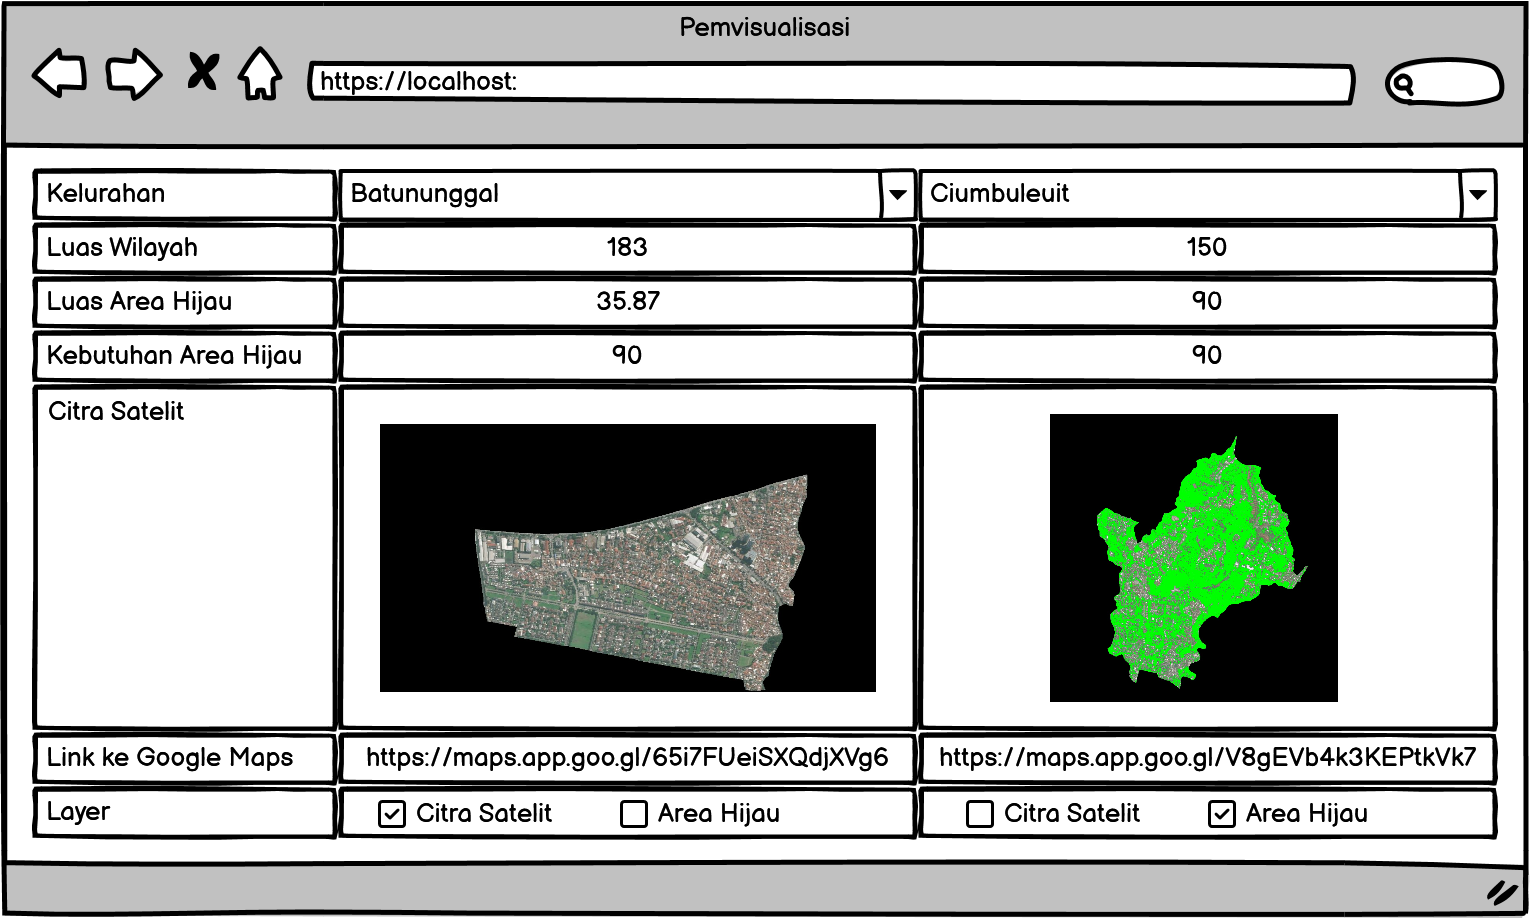
\includegraphics[width=0.8\textwidth]{perancangan.png}
			\caption{Rancangan Antarmuka}
			\label{fig:rancanganAntarmuka}
		\end{figure} 

		\item \textbf{Membangun laman web bedasarkan \textit{framework} Laravel}\\
		{\bf Status :} Ada sejak rencana kerja skripsi \\
		{\bf Hasil :} Proses pembangunan laman web bedasarkan \textit{framework} Laravel telah dilakukan. Hasil dari proses implementasi antarmuka perangkat lunak 'Pemvisualisasi Kelurahan Kota Bandung' dapat di lihat pada gambar \ref{fig:home1}.
			\begin{figure}[H]
				\centering
				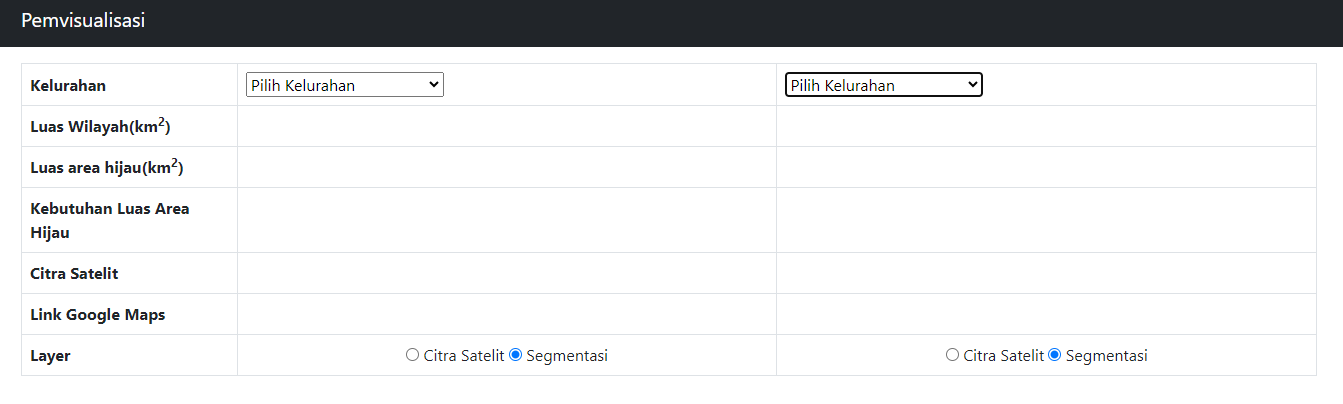
\includegraphics[width=0.8\textwidth]{home1.png}
				\caption{Antarmuka Halaman Utama}
				\label{fig:home1}
			\end{figure}
		
		Pengguna  memilih kelurahan yang ingin dilihat dengan cara menekan \textit{dropdown} yang akan menampilkan pilihan-pilihan kelurahan di kota Bandung. Implementasi antarmuka saat memilih kelurahan dapat dilihat pada  gambar \ref{fig:home2}.
			\begin{figure}[H]
				\centering
				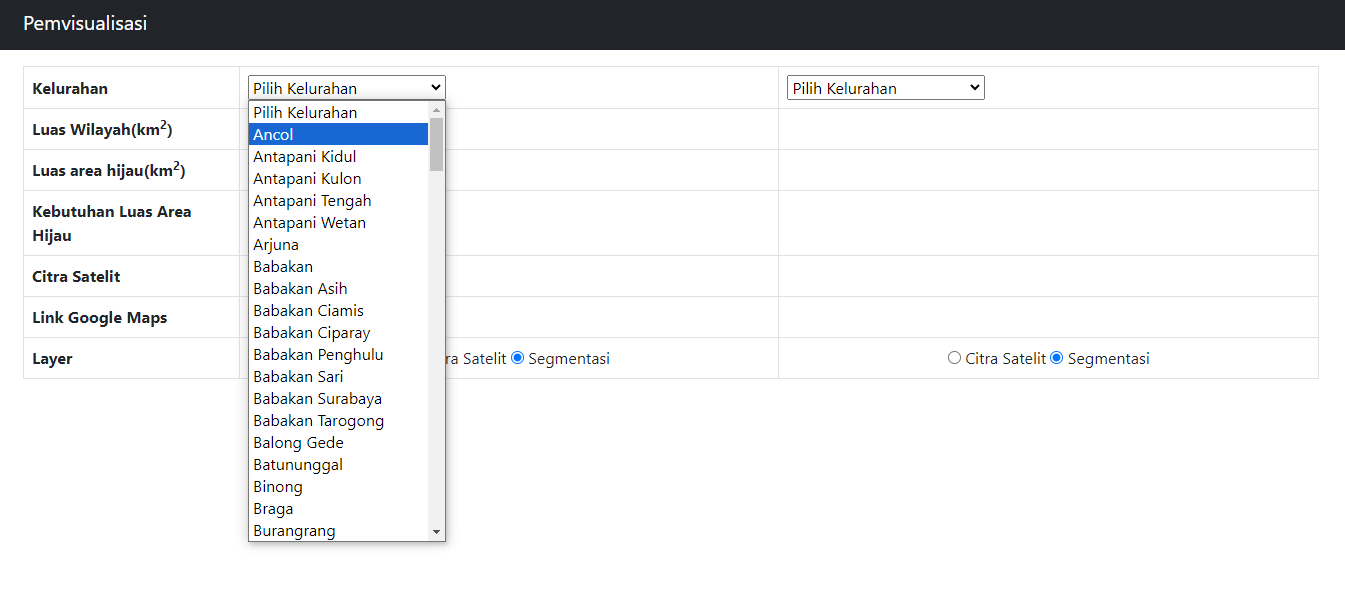
\includegraphics[width=0.8\textwidth]{home2.png}
				\caption{Antarmuka Halaman Utama (\textit{Dropdown})}
				\label{fig:home2}
			\end{figure} 
		Setelah pengguna memilih kelurahan maka perangkat lunak akan menampilkan data dari setiap kelurahan dapat dilihat pada gambar \ref{fig:home3}.
			\begin{figure}[H]
				\centering
				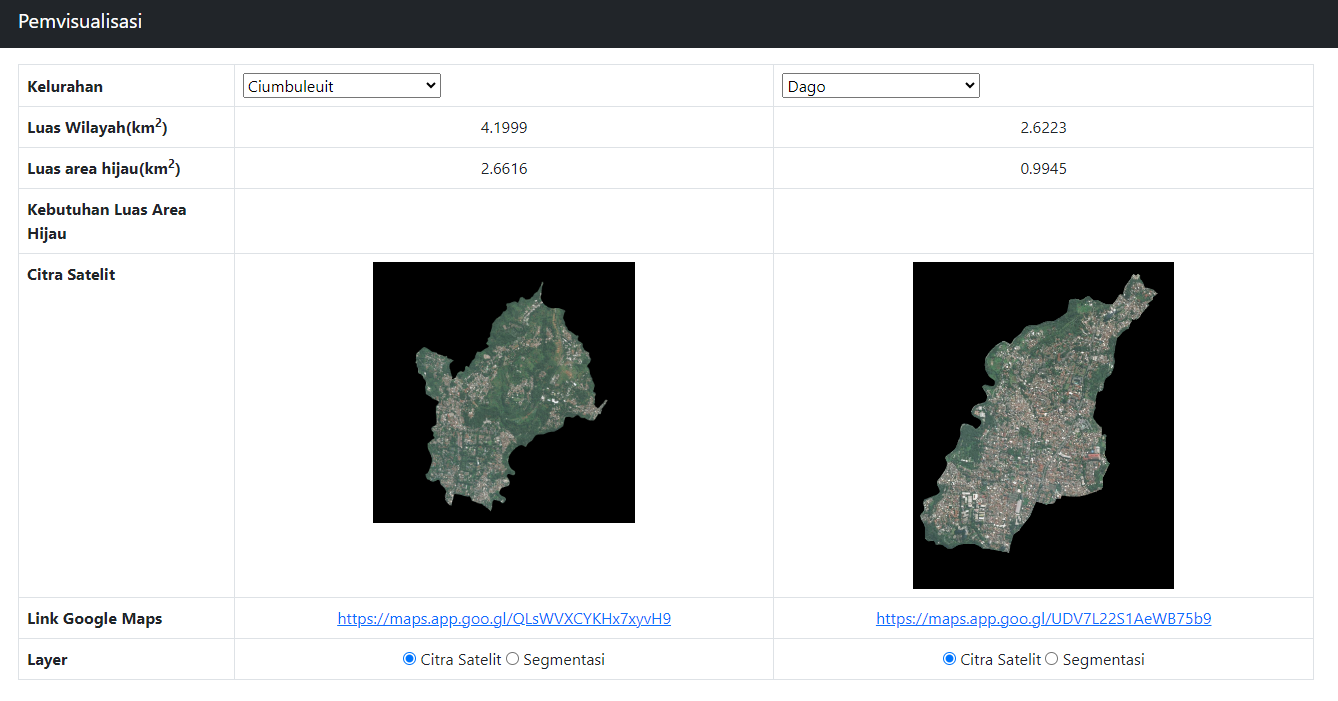
\includegraphics[width=0.8\textwidth]{home3.png}
				\caption{Antarmuka Halaman Utama Menampilkan Data Kelurahan}
				\label{fig:home3}
			\end{figure} 
		Pengguna dapat memilih gambar hasil segmentasi area hijau dengan cara menekan \textit{radio-button} segmentasi,  maka tampilan rancangan antarmuka akan dapat dilihat seperti pada gambar \ref{fig:home5}
			\begin{figure}[H]
				\centering
				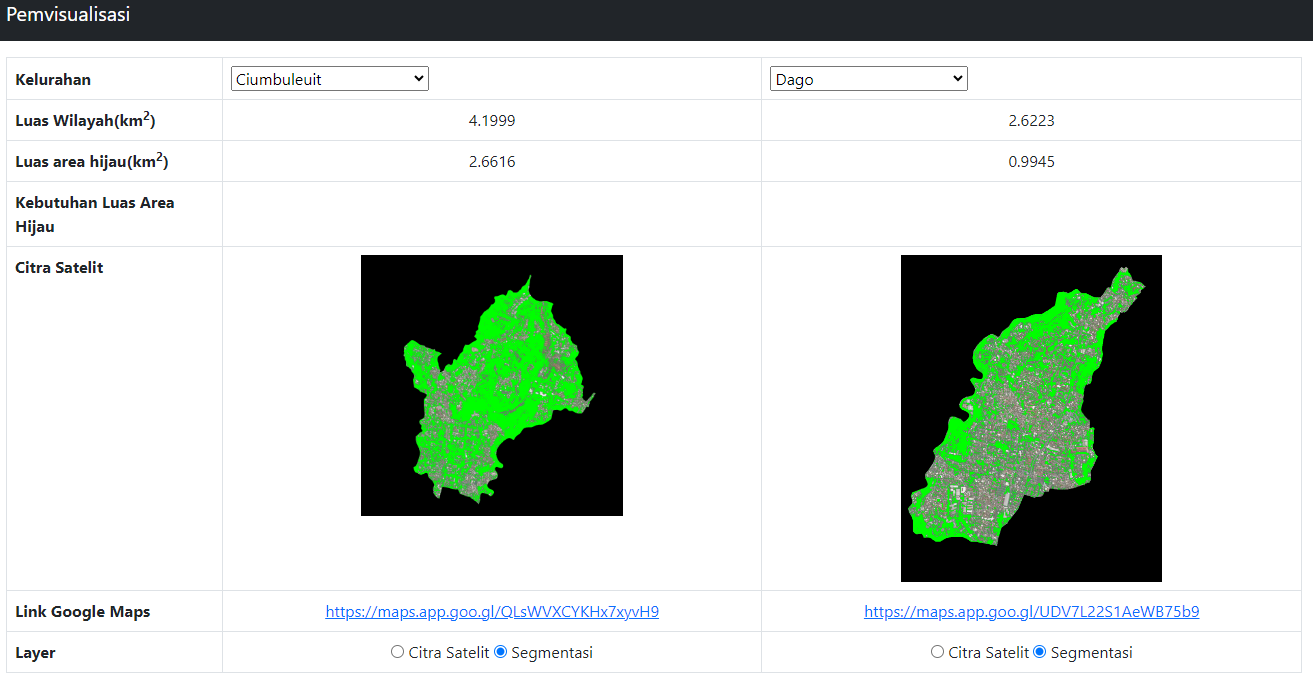
\includegraphics[width=0.8\textwidth]{home5.png}
				\caption{Antarmuka Halaman Utama Menampilkan Gambar Citra Satelit Segementai}
				\label{fig:home5}
			\end{figure} 
		
		\item \textbf{Melakukan pengujian pada laman web}\\
		{\bf Status :} Ada sejak rencana kerja skripsi \\
		{\bf Hasil :} Proses pengujian perangkat  lunak belum semuanya diselesaikan. Pengujian yang telah dilakukan adalah pengujian fungsional dimana fitur-fitur perangkat lunak yang dikembangkan dapat berjalan.  Hasil pengujian fungsional yang dilakukan terhadap dua buah kelurahan yaitu kelurahan Ciumbuleuit dan kelurahan Dago. Hasil pengujian fungsional yang dilakukan terhadap dua buah kelurahan yaitu kelurahan Ciumbuleuit dan kelurahan Dago dapat dilihat pada tabel \ref{tab:pengujian-fungsional-ciumbuleuit} dan tabel \ref{tab:pengujian-fungsional-dago}. Namun, pengujian eksperimental belum selesai dilakukan.
		\begin{table}[H]
			\centering
			\caption{Pengujian Fungsional Kelurahan Ciumbuleuit}
			\label{tab:pengujian-fungsional-ciumbuleuit}
			\resizebox{\textwidth}{!}{
				\begin{tabular}{|>{\hspace{0pt}}m{0.14\linewidth}|>{\hspace{0pt}}m{0.083\linewidth}|>{\hspace{0pt}}m{0.362\linewidth}|>{\hspace{0pt}}m{0.356\linewidth}|}
					\hline
					\textbf{Nama Fungsi}                         & \textbf{Kelurahan}  & \textbf{Hasil yang Diharapkan}                                                                                                            & \textbf{Hasil Pengujian}                                                                                                                  \\ 
					\hline
					Memilih kelurahan                            & Ciumbuleuit & Dropdown berisikan nama-nama kelurahan dan dapat dipilih                                                                                  & Dropdown berisikan nama-nama kelurahan dan dapat dipilih                                                                                  \\ 
					\hline
					Menampilkan Luas Wilayah                     & Ciumbuleuit  & Perangkat lunak akan menampilkan informasi berupa luas wilayah kelurahan yang dipilih                                                     & Perangkat lunak menampilkan informasi berupa luas wilayah kelurahan yang dipilih                                                          \\ 
					\hline
					Menampilkan Luas Area Hijau                  & Ciumbuleuit  & Perangkat lunak akan menampilkan informasi berupa luas area hijau kelurahan  yang dipilih                                                 & Perangkat lunak menampilkan informasi berupa luas area hijau kelurahan yang dipilih                                                       \\ 
					\hline
					Menampilkan Kebutuhan Luas Area Hijau        & Ciumbuleuit  & Perangkat lunak akan menampilkan informasi berupa kebutuhan luas area hijau kelurahan yang dipilih                                        & Perangat lunak belum bisa menampilkan informasi berupa kebutuhan luas area hijau kelurahan yang dipilih                                   \\ 
					\hline
					Menampilkan Gambar Citra Satelit             & Ciumbuleuit  & Perangkat lunak akan menampilkan gambar dari kelurahan                                                                                    & Perangkat lunak menampilkan gambar dari kelurahan yang dipilih                                                                            \\ 
					\hline
					Menampilkan Link Google Maps                 & Ciumbuleuit  & Perangkat lunak akan menampilkan link google maps dan jika ditekan akan alihkan kehalaman googlemaps sesuai dengan kelurahan yang dipilih & Perangkat lunak menampilkan link google maps dan jika ditekan akan dialihkan ke halaman google maps sesuai dengan kelurahan yang dipilih  \\ 
					\hline
					Menampilkan Gambar Segemetasi  Citra Satelit & Ciumbuleuit  & Perangkat lunak akan menampilkan gambar segmentasi citra satelit pada saat radio button segmentasi ditekan                                & Perangkan lunak menampilkan gambar segmentasi citra satelit pada saat radio button segementasi ditekan                                    \\
					\hline
				\end{tabular}
			}
		\end{table}
		
		\begin{table}[H]
			\centering
			\caption{Pengujian Fungsional Kelurahan Dago}
			\label{tab:pengujian-fungsional-dago}
			\resizebox{\textwidth}{!}{
				\begin{tabular}{|>{\hspace{0pt}}m{0.14\linewidth}|>{\hspace{0pt}}m{0.083\linewidth}|>{\hspace{0pt}}m{0.362\linewidth}|>{\hspace{0pt}}m{0.356\linewidth}|}
					\hline
					\textbf{Nama Fungsi}                         & \textbf{Kelurahan}  & \textbf{Hasil yang Diharapkan}                                                                                                            & \textbf{Hasil Pengujian}                                                                                                                  \\ 
					\hline
					Memilih kelurahan                            & Dago & Dropdown berisikan nama-nama kelurahan dan dapat dipilih                                                                                  & Dropdown berisikan nama-nama kelurahan dan dapat dipilih                                                                                  \\ 
					\hline
					Menampilkan Luas Wilayah                     & Dago  & Perangkat lunak akan menampilkan informasi berupa luas wilayah kelurahan yang dipilih                                                     & Perangkat lunak menampilkan informasi berupa luas wilayah kelurahan yang dipilih                                                          \\ 
					\hline
					Menampilkan Luas Area Hijau                  & Dago  & Perangkat lunak akan menampilkan informasi berupa luas area hijau kelurahan  yang dipilih                                                 & Perangkat lunak menampilkan informasi berupa luas area hijau kelurahan yang dipilih                                                       \\ 
					\hline
					Menampilkan Kebutuhan Luas Area Hijau        & Dago  & Perangkat lunak akan menampilkan informasi berupa kebutuhan luas area hijau kelurahan yang dipilih                                        & Perangat lunak belum bisa menampilkan informasi berupa kebutuhan luas area hijau kelurahan yang dipilih                                   \\ 
					\hline
					Menampilkan Gambar Citra Satelit             & Dago  & Perangkat lunak akan menampilkan gambar dari kelurahan                                                                                    & Perangkat lunak menampilkan gambar dari kelurahan yang dipilih                                                                            \\ 
					\hline
					Menampilkan Link Google Maps                 & Dago  & Perangkat lunak akan menampilkan link google maps dan jika ditekan akan alihkan kehalaman googlemaps sesuai dengan kelurahan yang dipilih & Perangkat lunak menampilkan link google maps dan jika ditekan akan dialihkan ke halaman google maps sesuai dengan kelurahan yang dipilih  \\ 
					\hline
					Menampilkan Gambar Segemetasi  Citra Satelit & Dago  & Perangkat lunak akan menampilkan gambar segmentasi citra satelit pada saat radio button segmentasi ditekan                                & Perangkan lunak menampilkan gambar segmentasi citra satelit pada saat radio button segementasi ditekan                                    \\
					\hline
				\end{tabular}
			}
		\end{table}
		
		
		
		\item \textbf{Menulis dokumen skripsi}\\
		{\bf Status :} Ada sejak rencana kerja skripsi.\\
		{\bf Hasil :} Hasil dari penulisan dokumen skripsi terdiri dari Bab 1 dan Bab 2. Dokumentasi skripsi bab 1 berisikan latar belakang, rumusan masalah, tujuan, batasan masalah, metodologi, dan sistematika pembahasan dari pemvisualisasi hasil penelitian area hijau kelurahan atau kecamatan. Sedangkan dokumentasi skripsi pada bab 2 berisikan penjelasan teori-teori yang akan digunakan dalam membangun perangkat lunak. Penjelasan teori-teori yang digunakan antara lain yaitu \textit{Command-line interface} pada terminal, \textit{Haddop Distributed File System}, \textit{Python} dengan \textit{library PIL(Pillow)}, \textit{base64}, dan \textit{Framework} Laravel. Pada bab 3 berisikan penjelasan mengenai proses pengumpulan data citra satelit yang berada di Laboratium Fakultas Tenik Informatika dan Sains(FTIS) UNPAR(Universitas Katolik Parahyangan) beserta gambar citra satelit segmentasi, pengambilan data dari hasil penelitian yang telah dilakukan oleh Juan A. Kusnandji, dan analisis kebutuhan perangkat lunak dalam pengembangan halaman web. Pada Bab 4 berisikan penjelaskan mengenai perancangan yang digunakan dalam membangun perangkat lunak. Pada bab 5 beriskan pembahasan tentang hasil dari rancangan antarmuka yang telah dibahas pada bab 4. Pengimplementasian rancangan antarmuka agar dapat menampilkan perbandingan visual antara dua kelurahan di kota Bandung. Juga akan membahas tentang pengujian fungsional,dan untuk pengujian eksperimental masih belum dilakukan. Pada bab 6 akan berisikan kesimpulan dan saran dalam pengembangan perangkat lunak namun pada bab ini masih belum diselesaikan.

		\item \textbf{Melakukan studi literatur dan studi eksplorasi mengenai \textit{Base64}}\\
		{\bf Status :} Baru ditambahkan pada skripsi 1.\\
		{\bf Hasil :} Mempelajari algoritma Base64 yang digunakan untuk mengubah tipe data \textit{bytes} menjadi tipe data yang dapat dilihat(dan sebaliknya). Pada penggunaan base64 telah terdapat pada \textit{library} dari bahasa pemrograman \textit{python} yang tinggal digunakan. Dalam penggunaan base64 pada \textit{script} pengekstraksian gambar dilakukan dengan men-\textit{decode} text menjadi format file ".png".
	\end{enumerate}
\newpage

\section{Pencapaian Rencana Kerja}
Langkah-langkah kerja yang berhasil diselesaikan dalam Skripsi 1 ini adalah sebagai berikut:
\begin{enumerate}
	\item Melakukan survei kepada Fritz H. Hutapea SKom dan Juan A. Kusjadi terkait penenilitiannya
	\item Melakukan pengumpulan data hasil penelitian
	\item Melakukan studi literatur dan studi eksplorasi mengenai Apache Hadoop
	\item Mempelajari ekstraksi data citra satelit yang disimpan pada HDFS
	\item Melakukan studi literatur dan studi eksplorasi mengenai \textit{Base64}
	\item Melakukan analisis kebutuhan laman web.
	\item Menulis dokumen skripsi
\end{enumerate}

Langkah-langkah kerja yang berhasil diselesaikan dalam Skripsi 2 ini adalah sebagai berikut:
\begin{enumerate}
	\item Mempelajari cara menggunakan \textit{framework} Laravel.
	\item Melakukan perancangan antarmuka laman web.
	\item Membangun laman web bedasarkan \textit{framework} Laravel
	\item Melakukan pengujian fungsional pada halaman web
	\item Menulis dokumen  skripsi
\end{enumerate}



\vspace{1cm}
\centering Bandung, \tanggal\\
%\vspace{2cm} 
\begin{figure}[h]
	\centering
	
\includegraphics[width=0.2\textwidth]{tandatangan.jpg}
\end{figure}
\nama \\ 
\vspace{1cm}

Menyetujui, \\
\ifdefstring{\jumpemb}{2}{
\vspace{1.5cm}
\begin{centering} Menyetujui,\\ \end{centering} \vspace{0.75cm}
\begin{minipage}[b]{0.45\linewidth}
% \centering Bandung, \makebox[0.5cm]{\hrulefill}/\makebox[0.5cm]{\hrulefill}/2013 \\
\vspace{2cm} Nama: \pembA \\ Pembimbing Utama
\end{minipage} \hspace{0.5cm}
\begin{minipage}[b]{0.45\linewidth}
% \centering Bandung, \makebox[0.5cm]{\hrulefill}/\makebox[0.5cm]{\hrulefill}/2013\\
\vspace{2cm} \pembB \\ Pembimbing Pendamping
\end{minipage}
\vspace{0.5cm}
}{
% \centering Bandung, \makebox[0.5cm]{\hrulefill}/\makebox[0.5cm]{\hrulefill}/2013\\
\vspace{2cm} \pembA \\ Pembimbing Tunggal
}
\end{document}

